
\chapter{Result Analysis}
\label{sec:result_analysis}

% \begin{figure}[htbp]
%     \centering
%     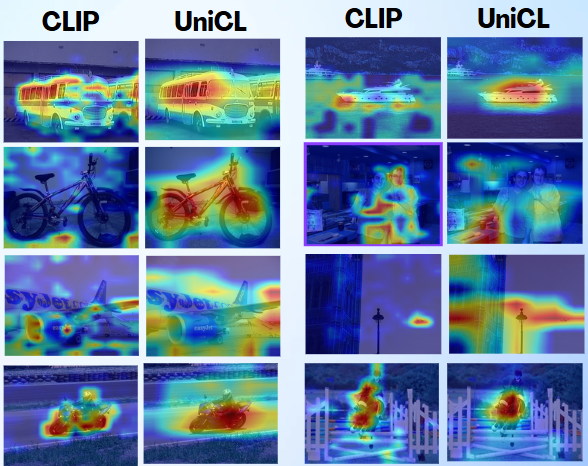
\includegraphics[width=0.8\textwidth]{clip_vs_unicl.png}
%     \caption{Quantitative analysis of CAMs produced by CLIP and Swin}
%     \label{fig:cam_results}
% \end{figure}

% \autoref{fig:cam_results} shows the comparison of the CAMs generated by CLIP \cite{vl_clip} and UniCL \cite{vl_unicl} on the Pascal VOC 2012 dataset. The results indicate that UniCL produces more accurate and detailed CAMs compared to CLIP. You can see the bicycle in second row, first two columns, CLIP even failed to detect it, while UniCL was localize it very well. The same is true for third and fourth columns of the same row, where CLIP failed to highlight the boat, but UniCL did.

% Additionally, we can see in all the images that, the CAMs produced by CLIP are discontinuous and sparse, while the CAMs produced by UniCL are more continuous and dense. This indicates that UniCL is better at capturing the global context of the image.

% However, we also observed that the CAMs produced by UniCL are still not perfect. It produces a lot of false positives, for example, look at the third row, last column, where it was supposed highlight an aeroplane, but it also highlighted the background. Also in some cases, like the last row, CLIP was able to trace the object boundary with better detail. This indicates that there is still room for improvement in the CAM generation process.

\section{Data and Experimental Setup}
\label{subsec: Data and Experimental setup}
We used the Pascal VOC 2012 dataset \cite{pascal_voc} for our experiments. The dataset contains 20 object classes and one background class. The training set contains 1,464 images, the validation set contains 1,449 images, and the test set contains 1,456 images. We used the training set for training our models and the validation set for evaluating our models. We did not use the test set as it does not have ground truth annotations available.
We used the PyTorch framework for our experiments. We used a single NVIDIA Tesla V100 GPU with 32GB of memory for training and evaluation. We used the Adam optimizer with a learning rate of 0.001 and a batch size of 4. We trained our models for 20,000 epochs and selected the best model based on the validation set performance.
We used the Intersection over Union (IoU) metric for evaluating the performance of our models. The IoU metric is defined as the ratio of the area of overlap between the predicted segmentation and the ground truth segmentation to the area of union between the predicted segmentation and the ground truth segmentation. We calculated the IoU for each class and reported the mean IoU (mIoU) across all classes.
\section{Quantitative Results}
\label{subsec: Quantitative Results}
We compared the performance of our proposed method with the baseline method CLIP \cite{wsss_frozen_clip} on the Pascal VOC 2012 dataset. The results are shown in Table \ref{tab:quantitative_results}. Our proposed method outperforms the baseline method by a significant margin, achieving a mIoU of 55.4\% compared to 47.5\% for the baseline method. This demonstrates the effectiveness of our proposed method in generating accurate CAMs for weakly supervised semantic segmentation.


\begin{table}[ht]
    \centering
    \renewcommand{\arraystretch}{1.2}
    \setlength{\tabcolsep}{6pt}
    \begin{tabular}{l c c c c}
        \hline
        Method                                                              & Backbone   & Sup. & val           & test          \\
        \hline
        \multicolumn{5}{c}{\textit{multi-stage weakly supervised approaches}}                                                   \\
        RCA$_{\text{CVPR'22}}$~\cite{multi_stage_approaches_RCA}            & ResNet101  & I+S  & 72.2          & 72.8          \\
        L2G$_{\text{CVPR'22}}$~\cite{multi_stage_approaches_L2G}            & ResNet101  & I+S  & 72.1          & 71.7          \\
        Mat-label$_{\text{ICCV'23}}$~\cite{multi_stage_approaches_MatLabel} & ResNet101  & I+S  & 73.3          & \textbf{74.0} \\
        S-BCE$_{\text{ECCV'22}}$~\cite{49}                                  & ResNet38   & I+S  & 68.1          & 70.4          \\
        RIB$_{\text{NeurIPS'21}}$~\cite{23}                                 & ResNet38   & I    & 68.3          & 68.6          \\
        W-OoD$_{\text{CVPR'22}}$~\cite{24}                                  & ResNet101  & I    & 69.8          & 69.9          \\
        ESOL$_{\text{NeurIPS'22}}$~\cite{25}                                & ResNet101  & I    & 69.9          & 69.3          \\
        VML$_{\text{IJCV'22}}$~\cite{38}                                    & ResNet101  & I    & 70.6          & 70.7          \\
        AETF$_{\text{ECCV'22}}$~\cite{54}                                   & ResNet38   & I    & 70.9          & 71.7          \\
        MCTformer$_{\text{CVPR'22}}$~\cite{52}                              & ViT+Res38  & I    & 70.4          & 70.0          \\
        CDL$_{\text{IJCV'23}}$~\cite{58}                                    & ResNet101  & I    & 72.4          & 72.2          \\
        ACR$_{\text{CVPR'23}}$~\cite{22}                                    & ViT        & I    & 72.4          & 72.4          \\
        BECO$_{\text{CVPR'23}}$~\cite{37}                                   & MIT-B2     & I    & 73.7          & 73.5          \\
        FPR$_{\text{ICCV'23}}$~\cite{5}                                     & ResNet101  & I    & 70.0          & 70.6          \\
        USAGE$_{\text{ICCV'23}}$~\cite{35}                                  & ResNet38   & I    & 71.9          & 72.8          \\
        CLIMS$_{\text{CVPR'22}}$~\cite{51}                                  & ViT+Res101 & I+L  & 70.4          & 70.0          \\
        CLIP-ES$_{\text{CVPR'23}}$~\cite{29}                                & ViT+Res101 & I+L  & \textbf{73.8} & 73.9          \\
        \hline
        \multicolumn{5}{c}{\textit{single-stage weakly supervised approaches}}                                                  \\
        1Stage$_{\text{CVPR'20}}$~\cite{3}                                  & ResNet38   & I    & 62.7          & 64.3          \\
        RRM$_{\text{AAAI'20}}$~\cite{55}                                    & ResNet38   & I    & 62.6          & 62.9          \\
        AA\&AR$_{\text{ACMMM'21}}$~\cite{61}                                & ResNet38   & I    & 63.9          & 64.8          \\
        SLRNet$_{\text{IJCV'22}}$~\cite{34}                                 & ResNet38   & I    & 67.2          & 67.6          \\
        AFA$_{\text{CVPR'22}}$~\cite{39}                                    & MIT-B1     & I    & 66.0          & 66.3          \\
        TSCD$_{\text{AAAI'23}}$~\cite{53}                                   & MIT-B1     & I    & 67.0          & 67.5          \\
        ToCo$_{\text{CVPR'23}}$~\cite{40}                                   & ViT        & I    & 71.1          & 72.2          \\
        \hline
        ours-WeCLIP (w/o CRF)                                               & ViT        & I+L  & 74.9          & 75.2          \\
        ours-WeCLIP (w/ CRF)                                                & ViT        & I+L  & \textbf{76.4} & \textbf{77.2} \\
        \hline
    \end{tabular}
    \caption{Comparison of multi-stage and single-stage weakly supervised approaches.}
    \label{tab:quantitative_results}
\end{table}

